\documentclass[11pt]{article}
\usepackage{amsmath,amssymb,amsthm}
\usepackage{graphicx}
\usepackage[margin=1in]{geometry}
\usepackage{fancyhdr}
\usepackage{graphicx}
\usepackage{subcaption}
\usepackage{float}
\setlength{\parindent}{0pt}
\setlength{\parskip}{5pt plus 1pt}
\setlength{\headheight}{13.6pt}
\newcommand\question[2]{\vspace{.25in}\hrule\textbf{#1: #2}\vspace{.5em}\hrule\vspace{.10in}}
\renewcommand\part[1]{\vspace{.10in}\textbf{#1}}
\pagestyle{fancyplain}
\lhead{\textbf{\NAME\ (\ANDREWID)}}
\chead{\textbf{HW\HWNUM}}
\rhead{\today}

\begin{document}\raggedright
	\newcommand\NAME{Muhammed Burak Bugrul}
	\newcommand\ANDREWID{150140015}
	\newcommand\HWNUM{2}
	
	\textbf{Note:} Version of Wireshark program that used for this assignment is 2.6.5.
	\question{Q1}{DHCP}
	
	When connecting to a new network, 4 new type of DHCP requests occur. Here is a screenshot taken from wireshark program while connecting a new network.
	
	\begin{figure}[h!]
		\centering
		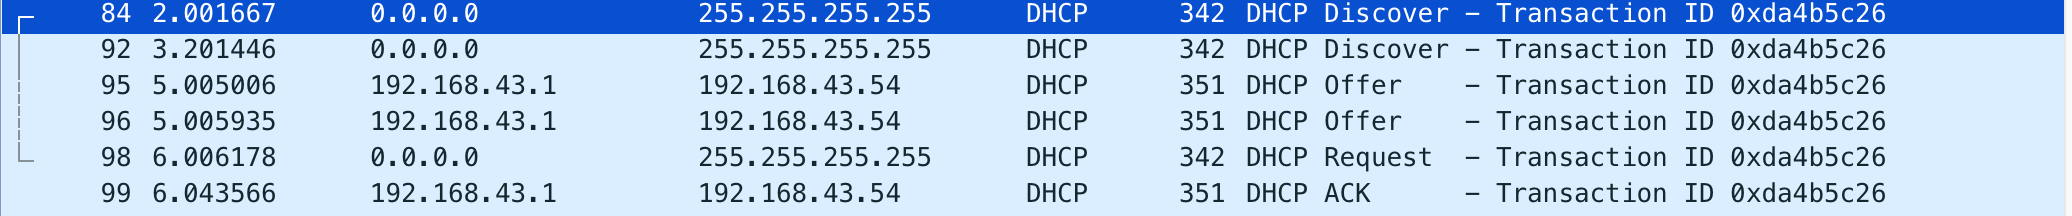
\includegraphics[width=0.5\textwidth]{images/dhcp-wireshark.png}
		\caption{DHCP}
		\label{fig:DHCP}
	\end{figure}

	These 4 type of requests are:\\ \ \\
	\textbf{DHCP DISCOVER:} A discover request that uses broadcast channel(FF.FF.FF.FF) for finding a DHCP server.\\
	\textbf{DHCP OFFER:} DHCP server decides whis addres to be given to the client and sends this address as an offer to the client.\\
	\textbf{DHCP REQUEST:} Client accepts the address.\\
	\textbf{DHCP ACKNOWLEDGEMENT:} Server confirms the acceptance.\\

	\begin{figure}[H]
		\centering
		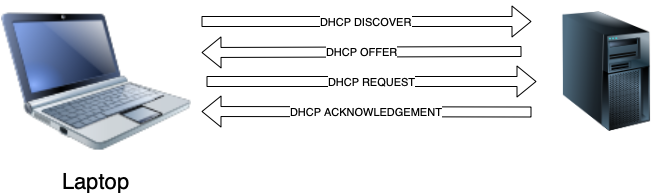
\includegraphics[width=0.5\textwidth]{images/dhcp-diagram.png}
		\caption{DHCP Diagram}
		\label{fig:DHCP Diagram}
	\end{figure}

	\question{Q2}{Video and Voice Traffic}
	
	\begin{figure}[H]
		\centering
		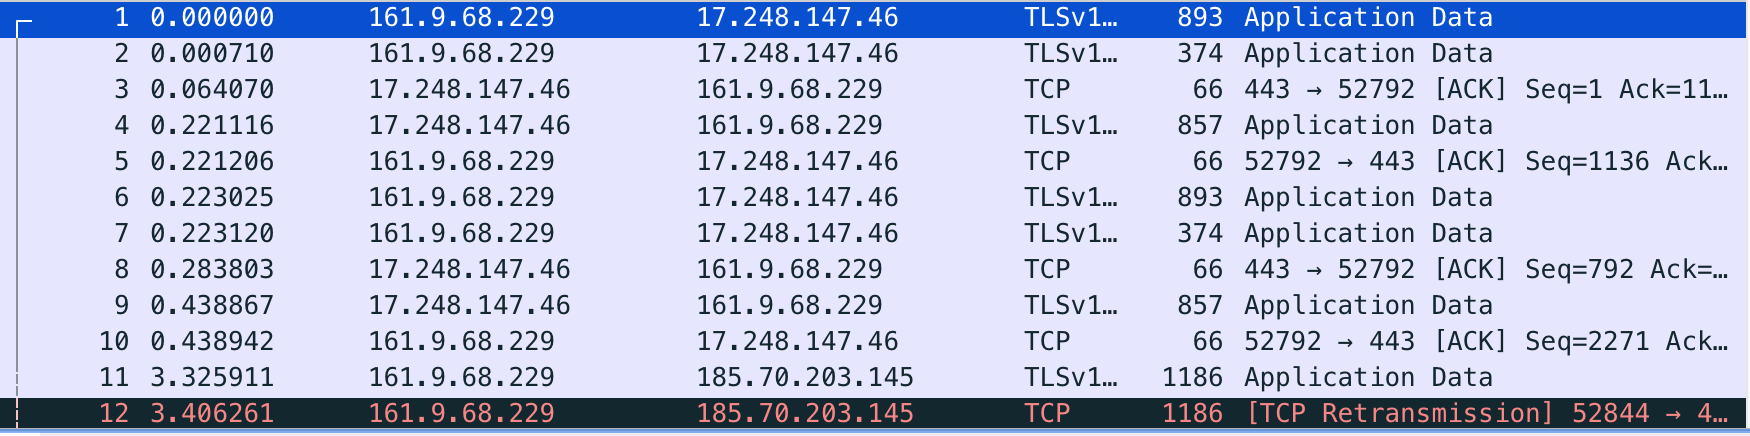
\includegraphics[width=0.5\textwidth]{images/video.png}
		\caption{Youtube}
		\label{fig:Youtube}
	\end{figure}

	There was no UDP connection from youtube.com nor another video website. Retransmissions occured in TCP because of lack of acknowledgement and timeout.
	
	\cleardoublepage

	\question{Q3}{Audio}
	
	\begin{figure}[H]
		\centering
		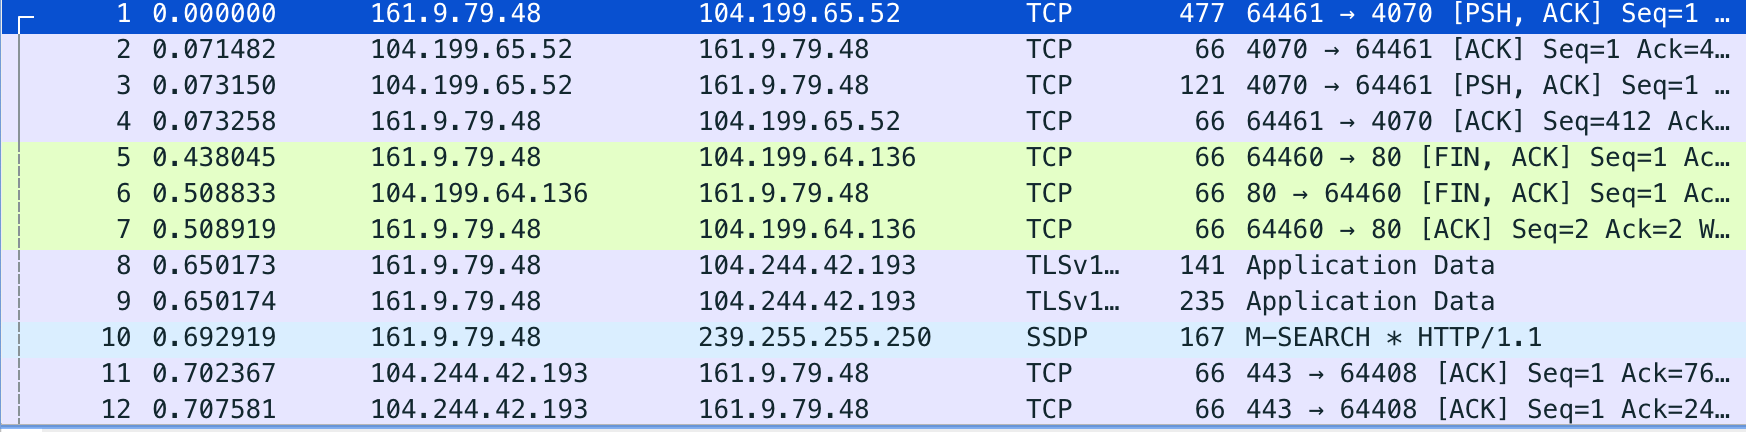
\includegraphics[width=0.5\textwidth]{images/audio-1.png}
		\caption{Audio-1}
		\label{fig:Audio-1}
	\end{figure}
	
	\begin{figure}[H]
		\centering
		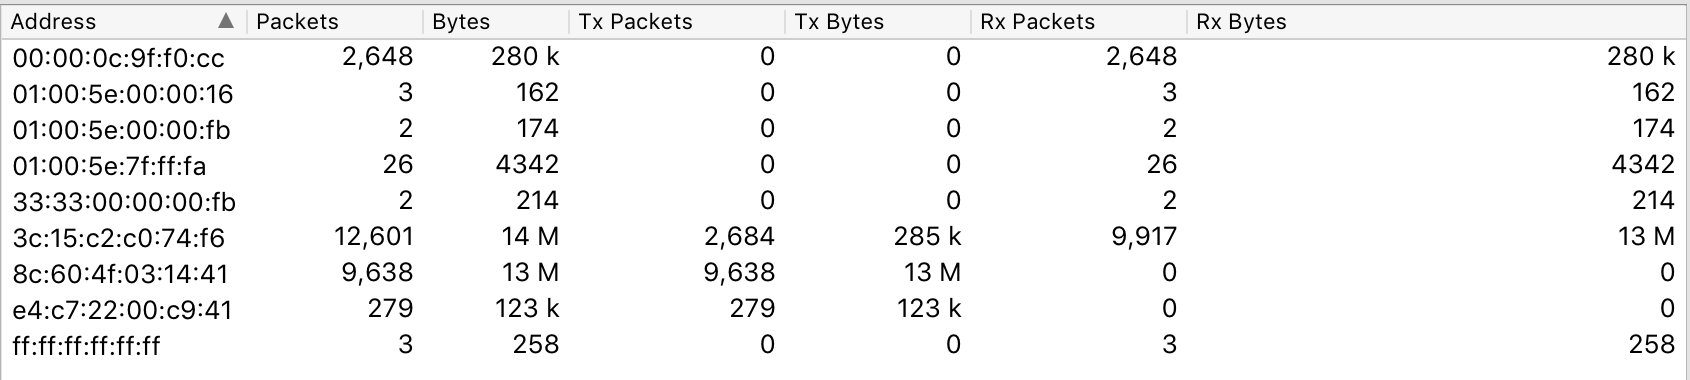
\includegraphics[width=0.5\textwidth]{images/audio-2.png}
		\caption{Audio-2}
		\label{fig:Audio-2}
	\end{figure}

	Statistics:
	
	\begin{figure}[H]
		\centering
		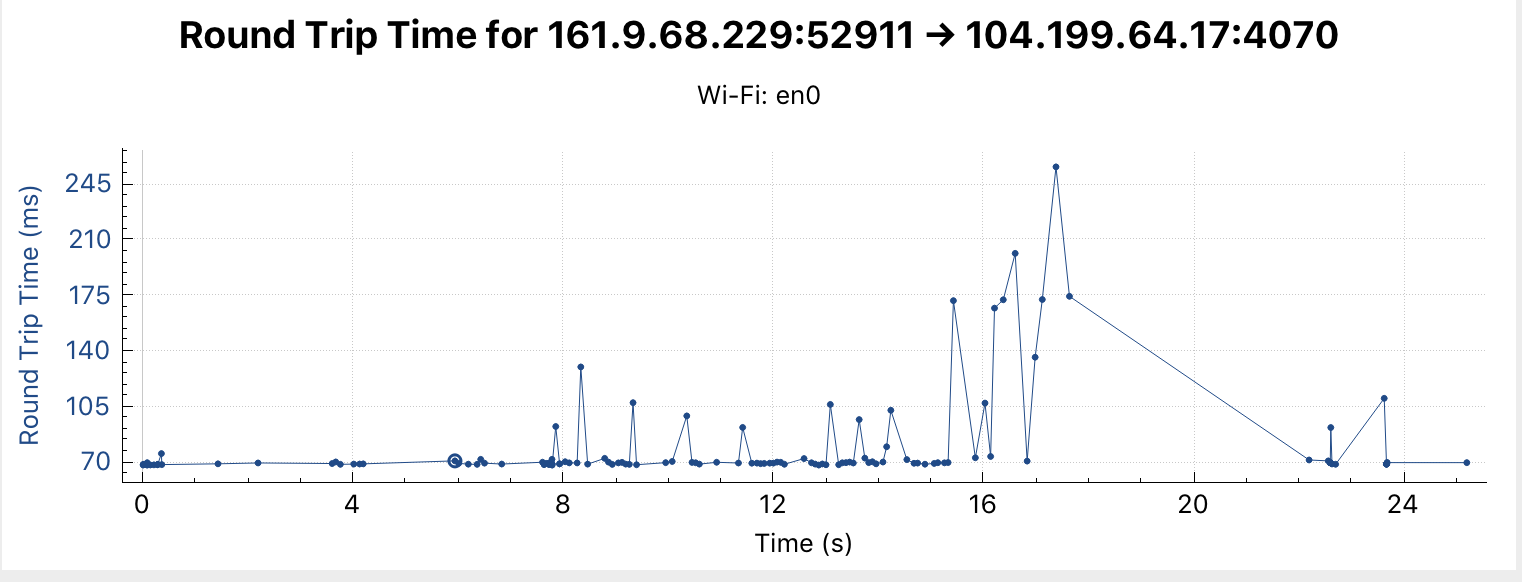
\includegraphics[width=0.5\textwidth]{images/rtt.png}
		\caption{RTT}
		\label{fig:RTT}
	\end{figure}

	\begin{figure}[H]
		\centering
		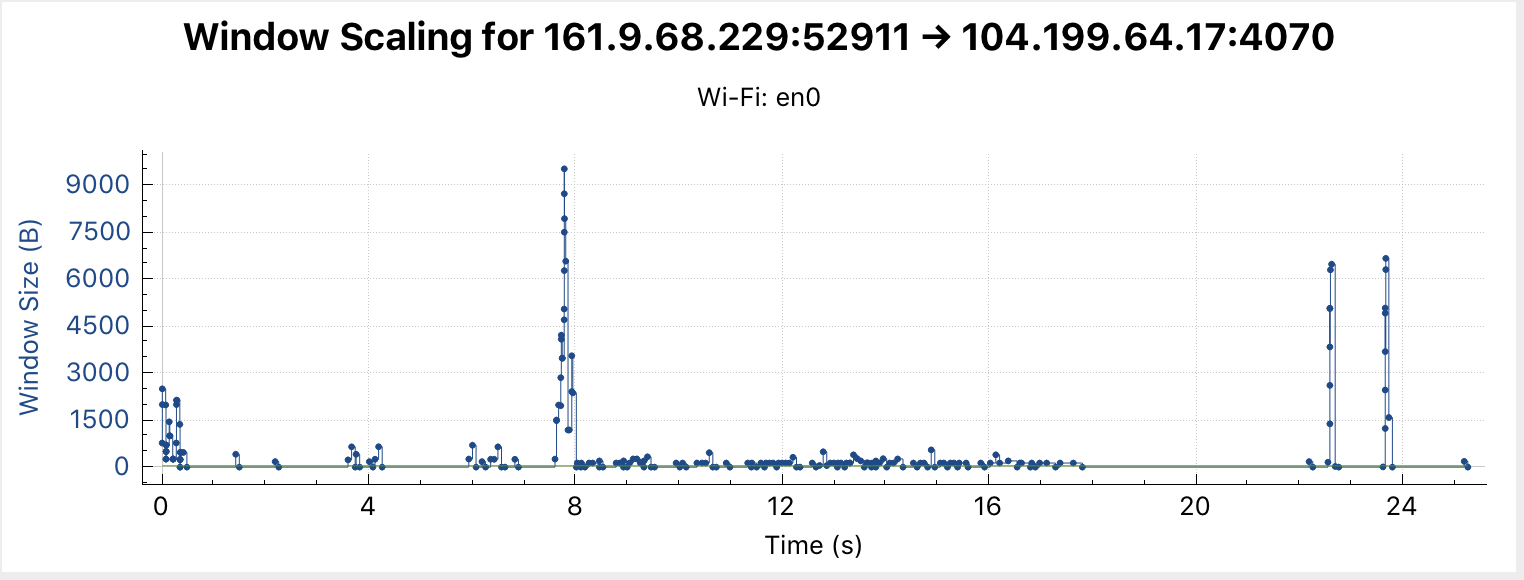
\includegraphics[width=0.5\textwidth]{images/window.png}
		\caption{Window}
		\label{fig:Window}
	\end{figure}

	\begin{figure}[H]
		\centering
		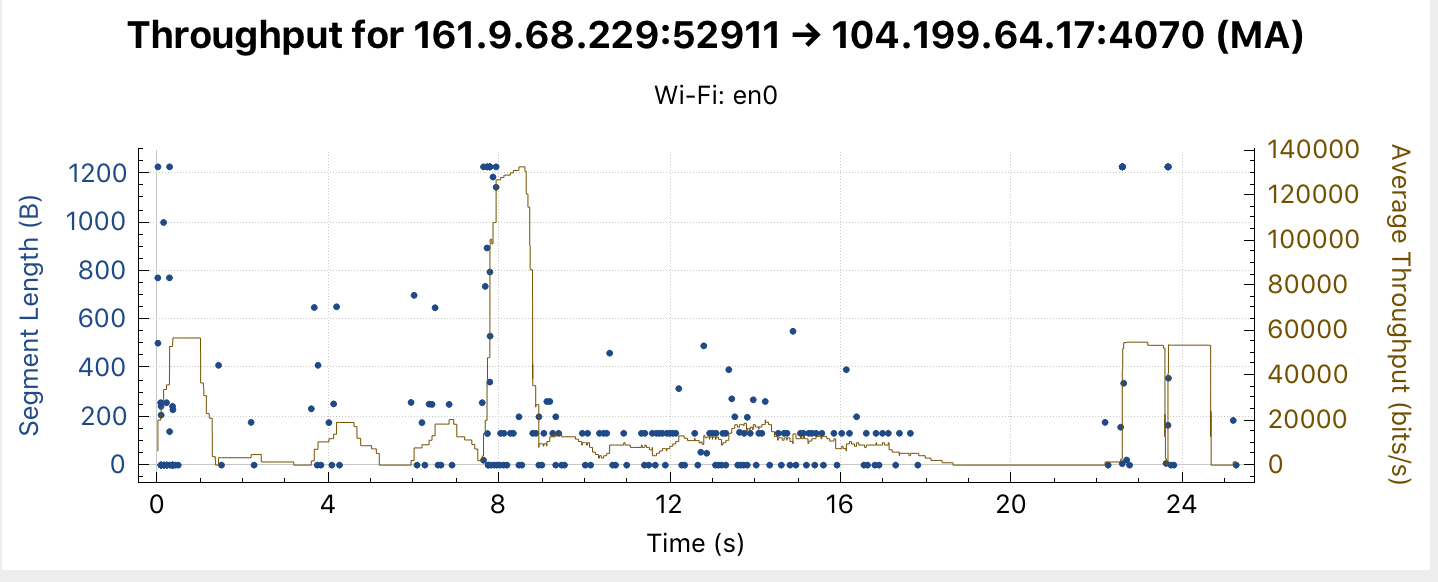
\includegraphics[width=0.5\textwidth]{images/throughput.png}
		\caption{Throughput}
		\label{fig:Throughput}
	\end{figure}

	\question{Q4}{FTP}
	Wireshark ss while it is watching file transfer:
	
	\begin{figure}[H]
		\centering
		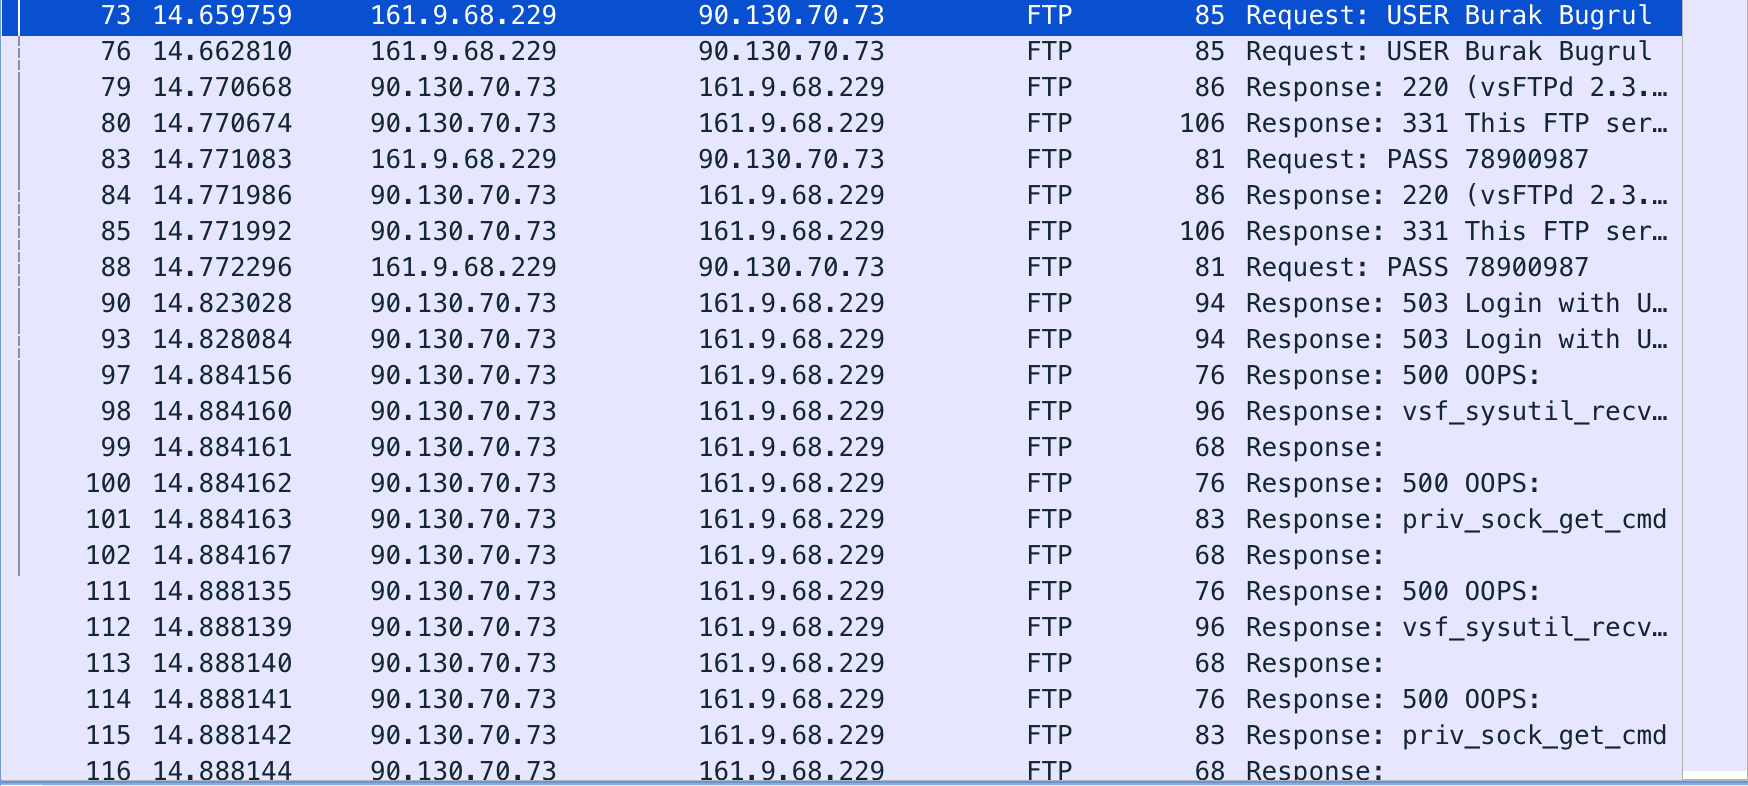
\includegraphics[width=0.5\textwidth]{images/ftp-1.png}
		\caption{FTP-1}
		\label{fig:FTP-1}
	\end{figure}
	\begin{figure}[H]
		\centering
		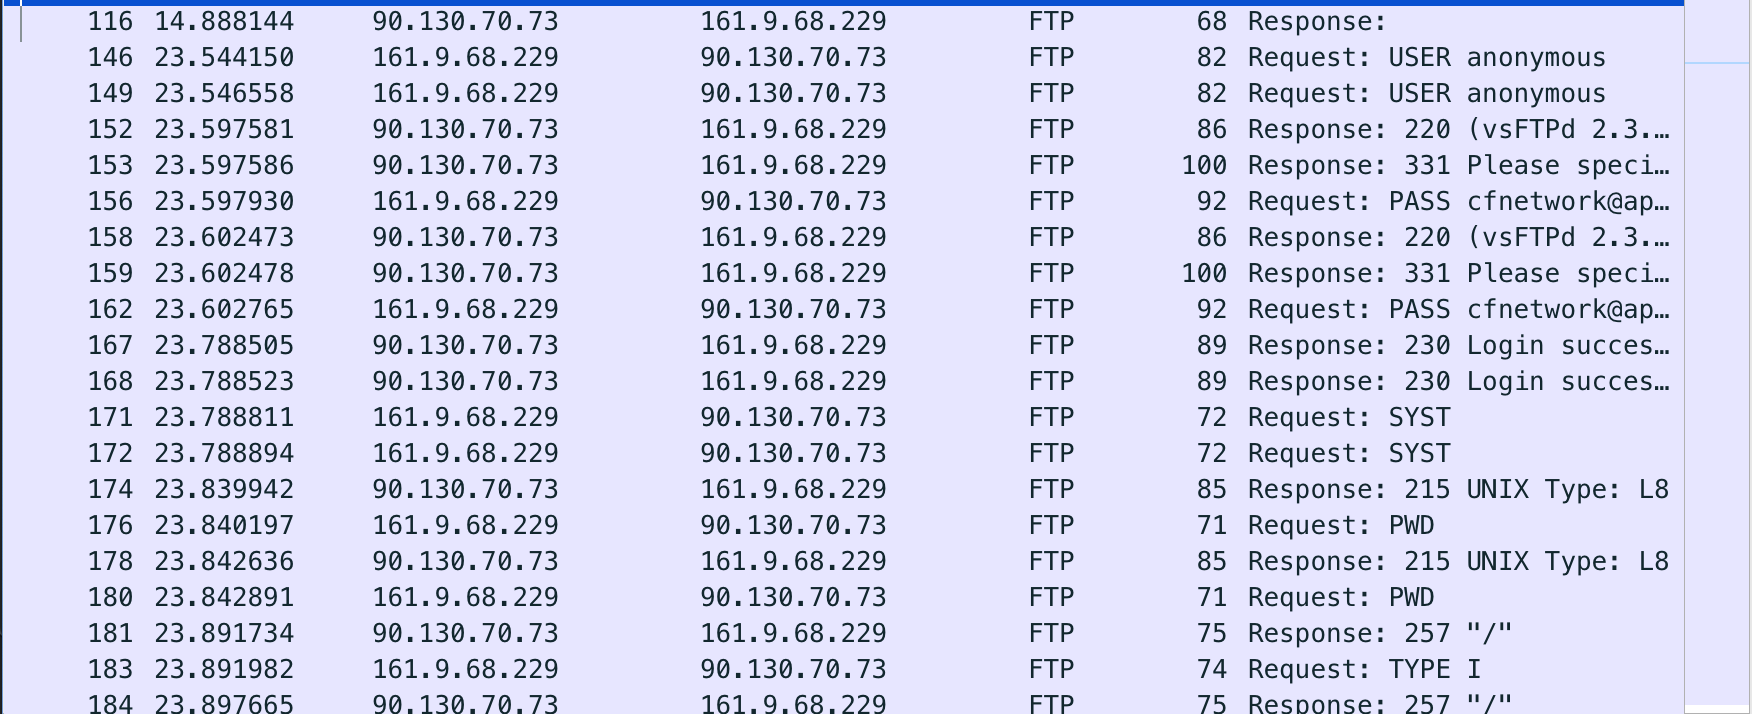
\includegraphics[width=0.5\textwidth]{images/ftp-2.png}
		\caption{FTP-2}
		\label{fig:FTP-2}
	\end{figure}
	\begin{figure}[H]
		\centering
		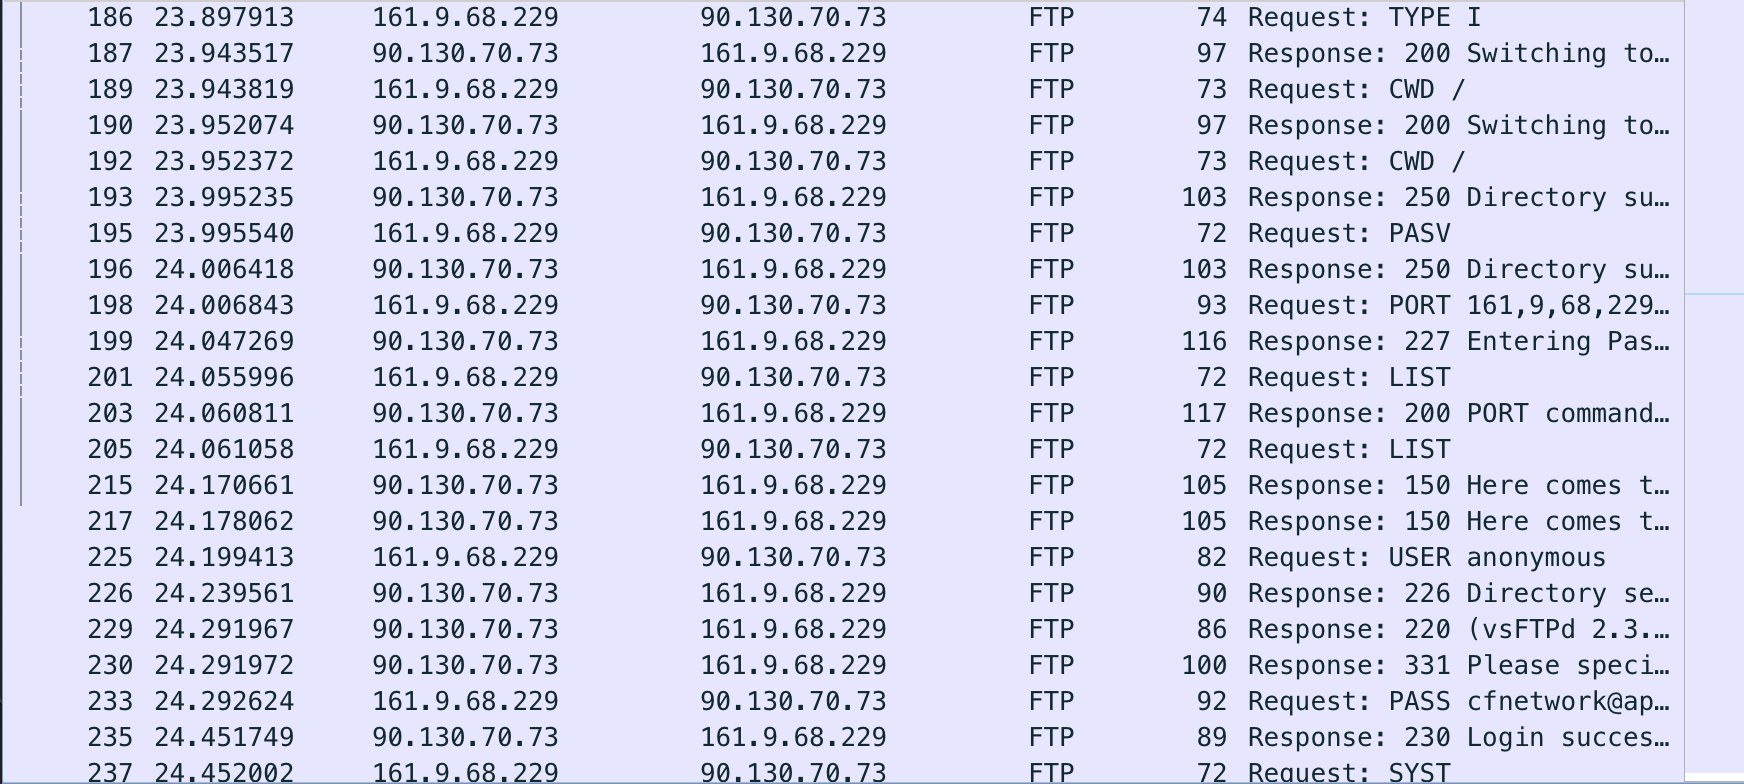
\includegraphics[width=0.5\textwidth]{images/ftp-3.png}
		\caption{FTP-3}
		\label{fig:FTP-3}
	\end{figure}
	\begin{figure}[H]
		\centering
		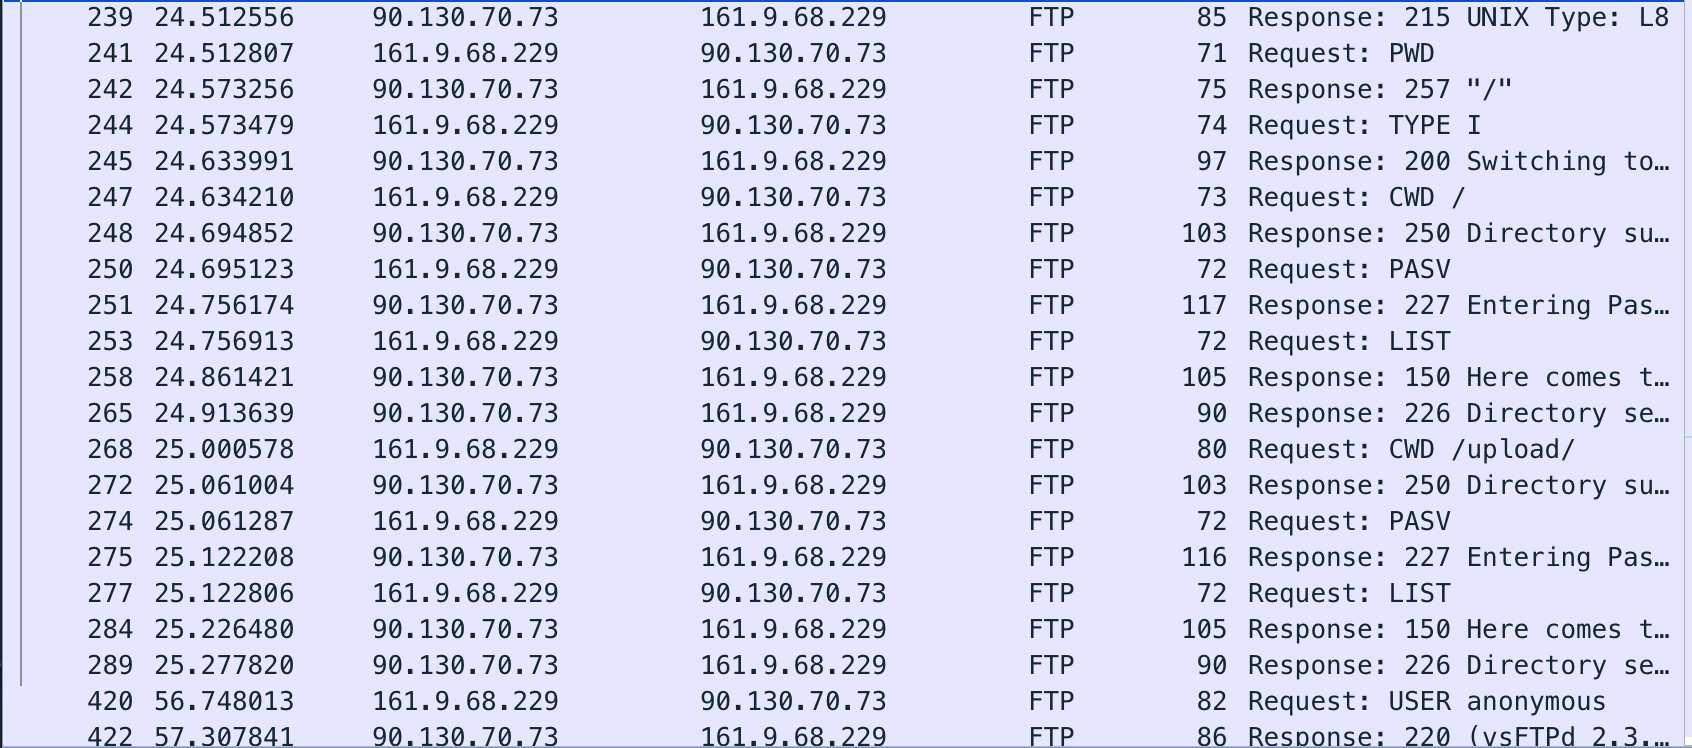
\includegraphics[width=0.5\textwidth]{images/ftp-4.png}
		\caption{FTP-4}
		\label{fig:FTP-4}
	\end{figure}
	\begin{figure}[H]
		\centering
		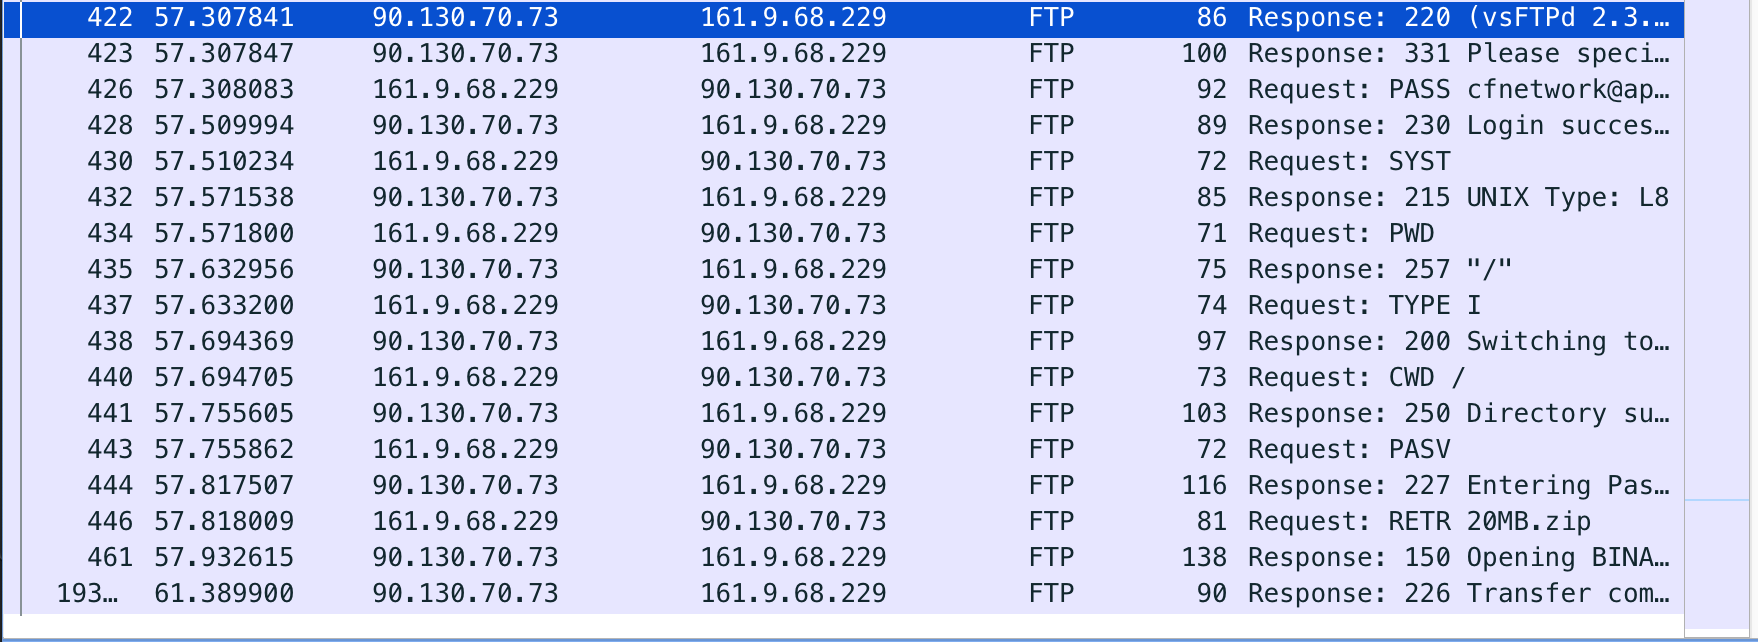
\includegraphics[width=0.5\textwidth]{images/ftp-5.png}
		\caption{FTP-5}
		\label{fig:FTP-5}
	\end{figure}

	In the beginning user wants to see the inside of the directory. Server sends it, then asks for username. User sends the usename and can not pass the auth. step. Server sends an error. Then user accesses the system as a guest. Server shows the files. Then users sends a dowload request. Server allows it and sends the file in packets.
	
	\question{Q5}{Protocols}
	\part{a)} Protocols that captured by Wireshark are: TCP, DNS, DHCP, TLS, FTP\\
	\part{b)}
	\begin{figure}[H]
		\centering
		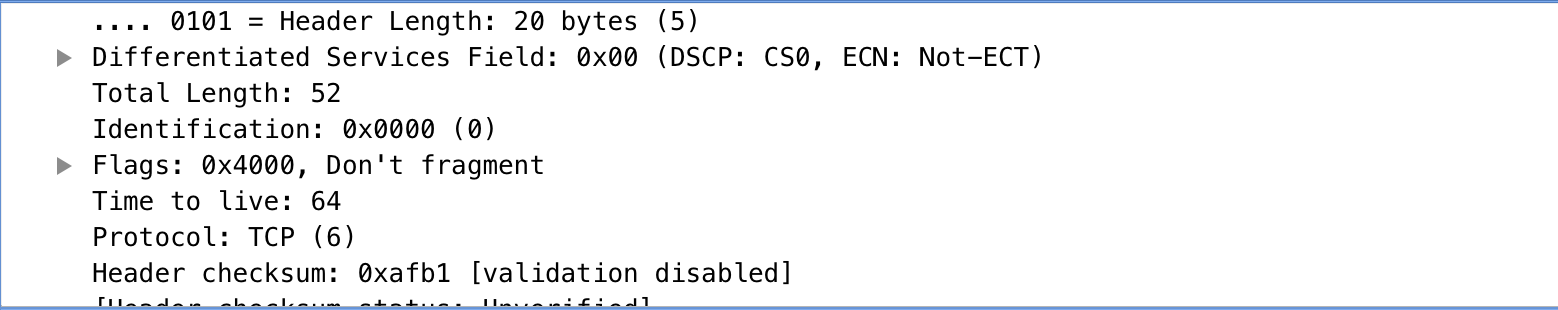
\includegraphics[width=0.5\textwidth]{images/tcp-number.png}
		\caption{TCP-NUMBER}
		\label{fig:TCP-NUMBER}
	\end{figure}

	Protocol number of TCP is 6.
	
	\begin{figure}[H]
		\centering
		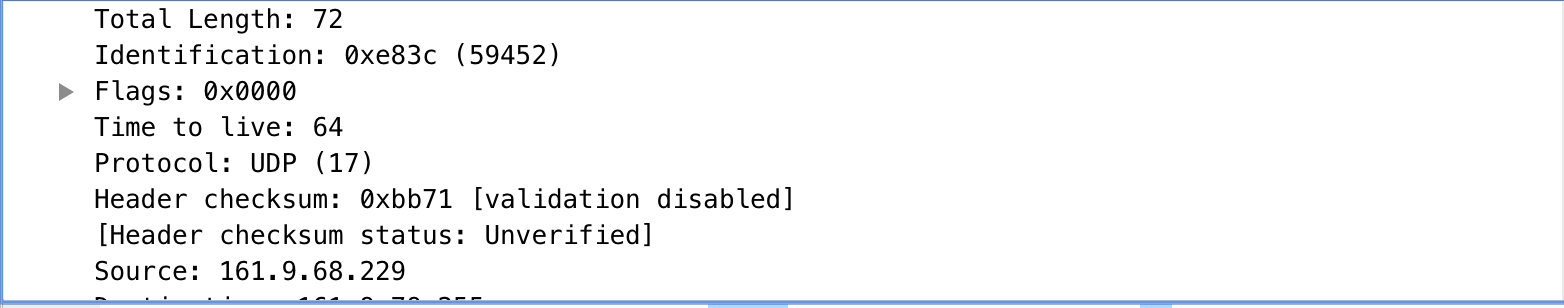
\includegraphics[width=0.5\textwidth]{images/udp-number.png}
		\caption{UDP-NUMBER}
		\label{fig:UDP-NUMBER}
	\end{figure}
	
	Protocol number of UDP is 17.
	
	\begin{figure}[H]
		\centering
		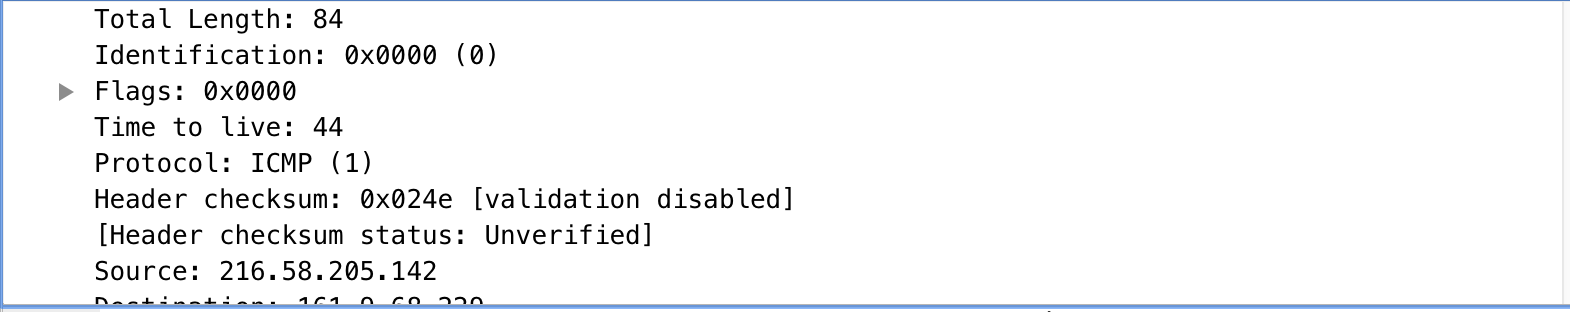
\includegraphics[width=0.5\textwidth]{images/icmp-number.png}
		\caption{ICMP-NUMBER}
		\label{fig:ICMP-NUMBER}
	\end{figure}
	
	Protocol number of ICMP is 1.
\end{document}